\chapter{Анализ данных эксперимента}\label{chapt:data_analysis}

После проведения экспериментальных исследований влияния радиуса закругления рабочей кромки и шага резания на составляющие силы, возникающей на дисковом инструменте, при механическом разрушении льда, получен набор <<сырых>> данных, который включает в себя:
\begin{itemize}
	\item фотографии осколков;
	\item фотографии образцов после проведения эксперимента;
	\item графики переходных процессов для каждого сочетания факторов.
\end{itemize}

Дальнейшее их использование предполагает обработку и оценку корректности методами математики и статистики, такими как:
\begin{itemize}
	\item отброс грубых ошибок;
	\item фильтрация:
	\begin{itemize}
		\item сглаживание;
		\item отброс постоянной составляющей;
	\end{itemize}		
%	\item оценка дисперсии;
	\item усреднение значений повторных экспериментов.		
\end{itemize}

Далее в это главе процесс обработки и оценки адекватности данных будет приведен последователь.

\section{Отброс грубых ошибок}\label{sect:drop_gross_error}

Для улучшения точности оценки переходного процесса и снижения влияния всевозможных внешних факторов целесообразно применить к полученному набору точек (сигналу) алгоритм отброса грубых ошибок \cite{LvovStat}. Суть алгоритма заключается в использовании метода максимального относительного отклонения:
\begin{equation}\label{eq:MOO}
\tau=\frac{|x_i-\bar{x}|}{\sigma_x},
\end{equation} 
где $ x_i $ "--- крайний (наибольший или наименьший) элемент сигнала; $ \bar{x} $ "--- среднее значение сигнала; $ \sigma_x $ "--- СКО сигнал (расчитывается по формуле \ref{eq:sigma_x}).

Сравнивая $ \tau $ с критическим значением $ \tau_{(p,n)} $, рассчитанным по формуле \ref{eq:tau_krit}, можно сделать вывод является ли наблюдение грубой погрешностью или нет.
\begin{equation}\label{eq:tau_krit}
\tau_{(p,\ n)}=\frac{t_{(p,\ n-2)}\cdot\sqrt{n-1}}{\sqrt{n-2+|t_{(p,\ n-2)}|^2}}
\end{equation}
где $ t_{(p,\ n-2)} $ "--- критическое значение распределения Стьюдента при доверительной вероятность $ q=1-p $; $ n $ "--- количество наблюдений в сигнале переходного процесса.

Критическое значение распределения Стьюдента в ППП matlab можно вычислить с помощью функции \lstinline{tinv()}. 
\begin{lstlisting}[stepnumber=0]
t = tinv(p / 100, n - 2);
\end{lstlisting}
где \lstinline{p} "--- вероятность; \lstinline{n} "--- количество наблюдений.

Таким образом имеем алгоритм отброса грубых ошибок представленный на рисунке \ref{img:AlgDGE}.

\begin{figure}[!ht]
	\center
	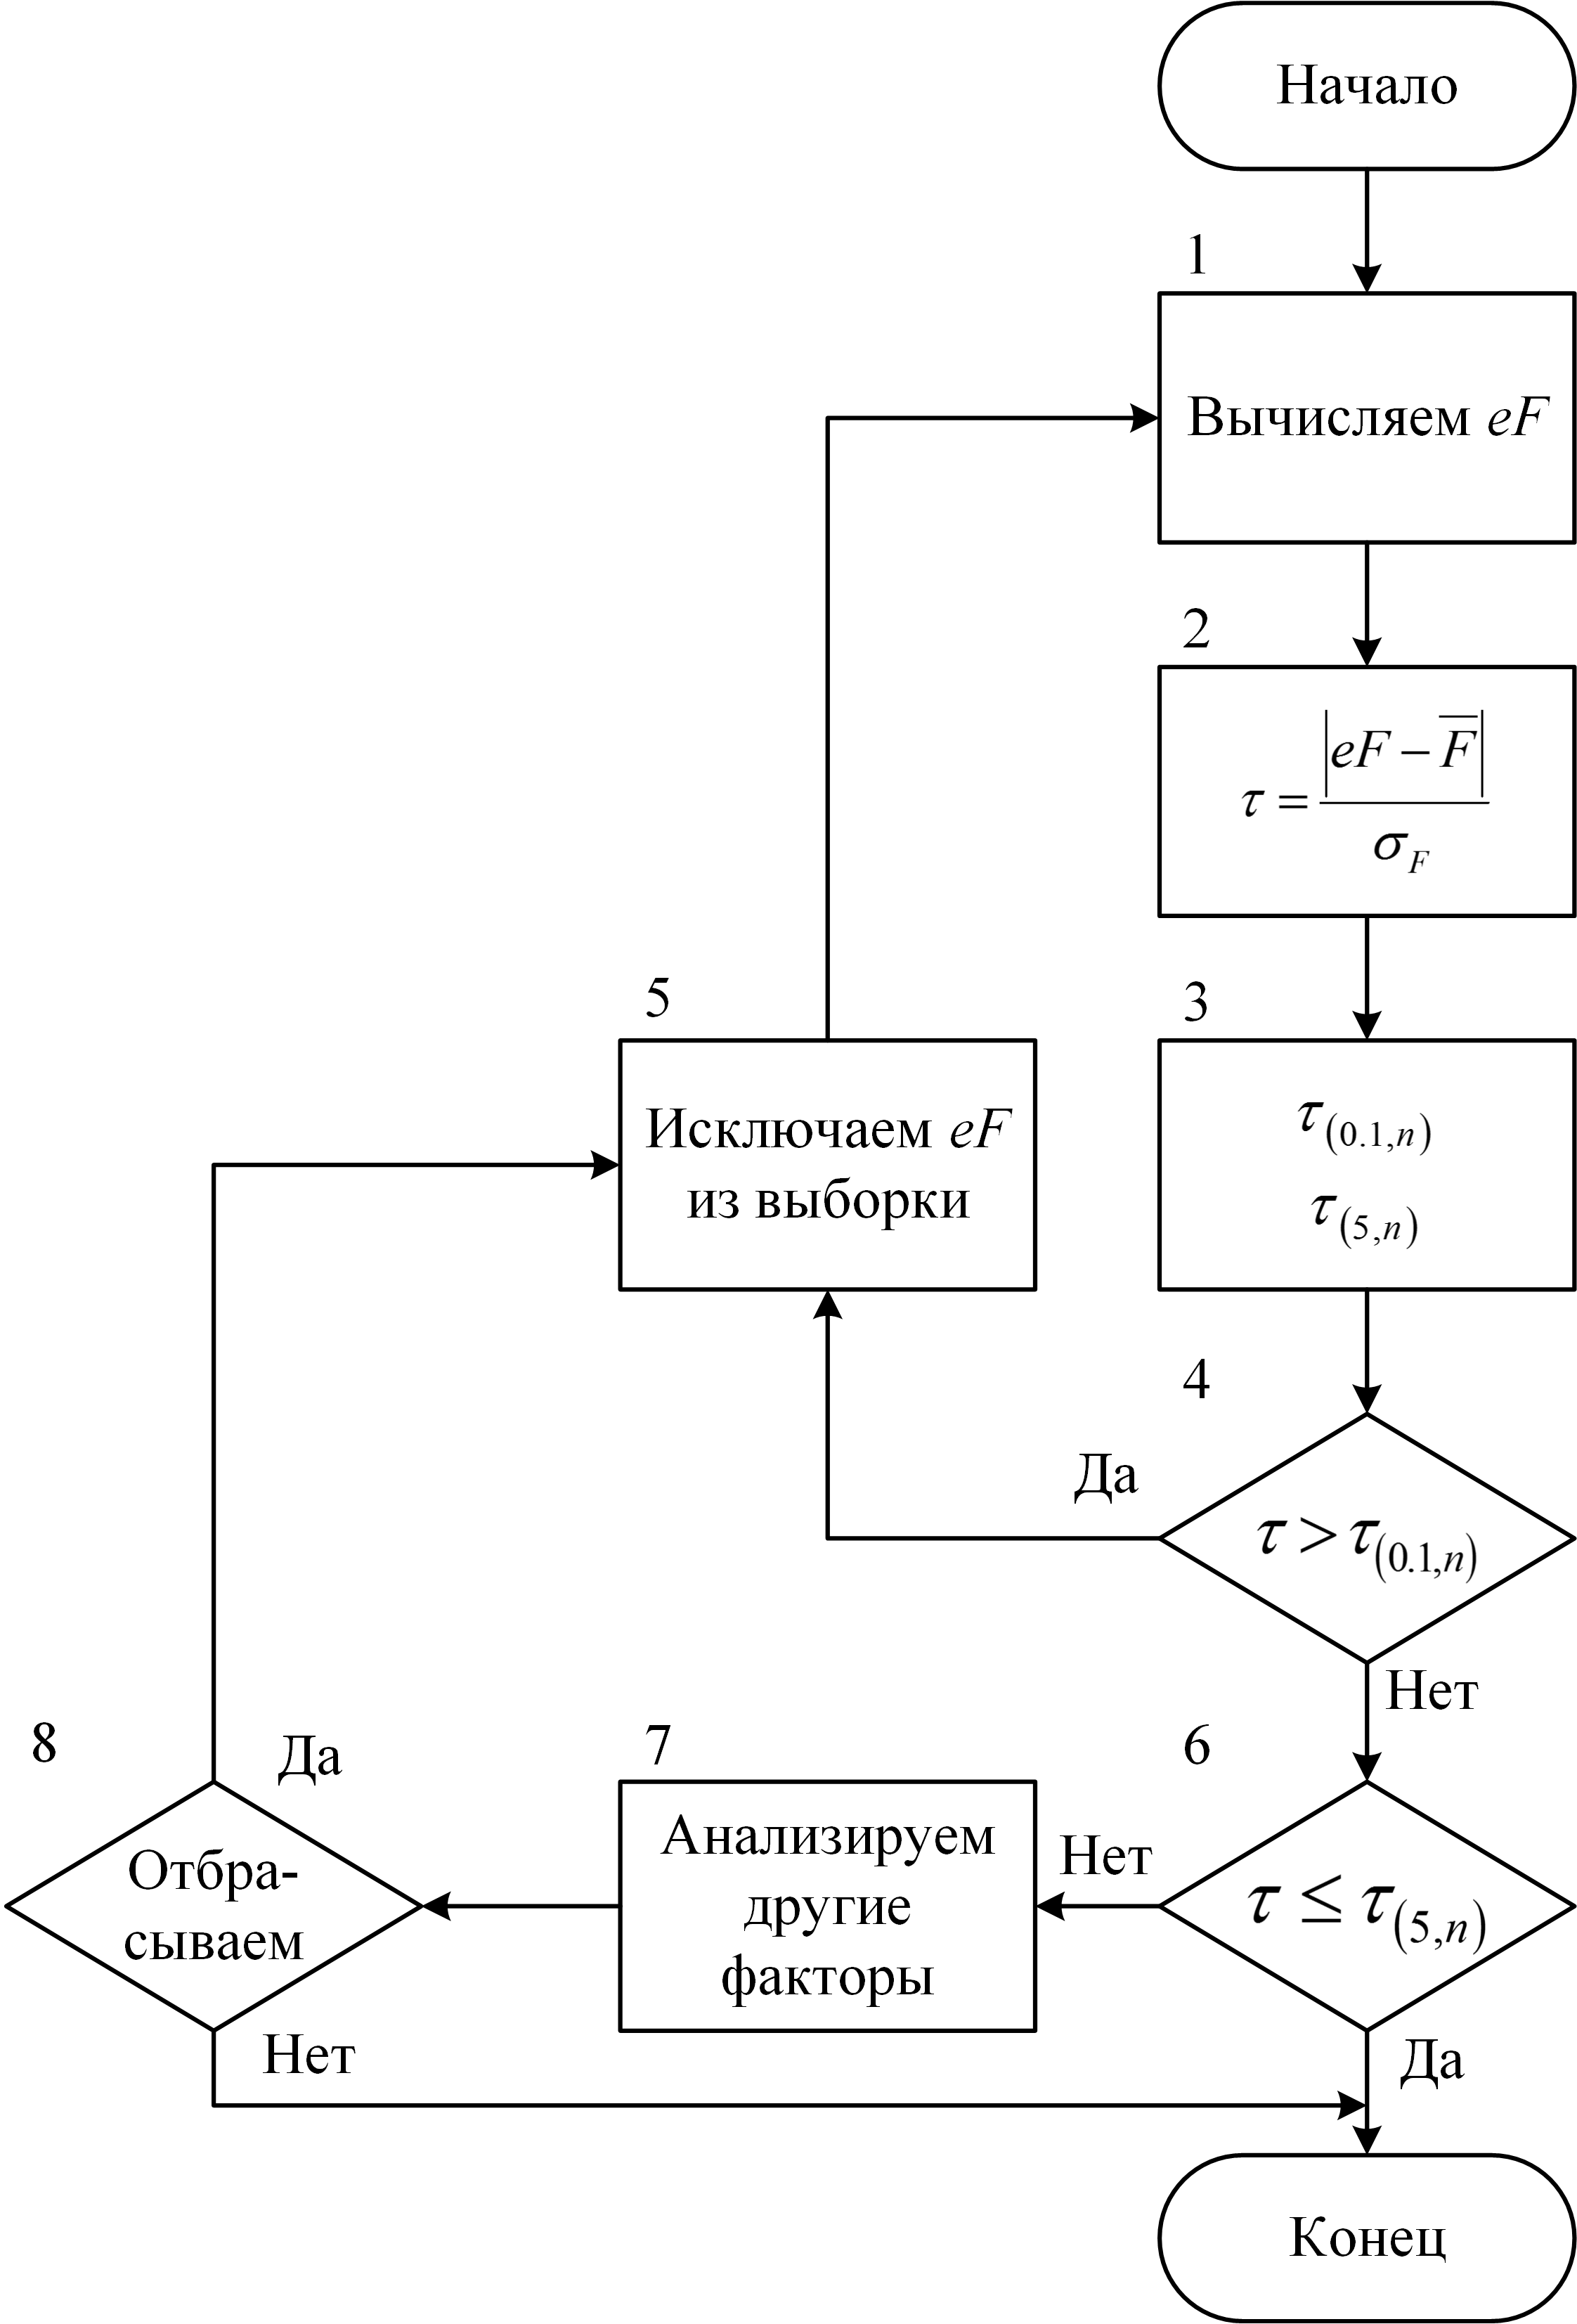
\includegraphics[scale=1.2]{DropGrossError}
	\caption{Алгоритм отброса грубых ошибок} 
	\label{img:AlgDGE}  
\end{figure}

Имеет смысл ввести три группы наблюдений, удовлетворяющих следующим условиям:
\begin{itemize}
	\item $ \tau \leqslant \tau_{(5\%,\ n)} $ нельзя отсеивать.
	\item $ \tau_{(5\%,\ n)} < \tau < \tau_{(0,1\%,\ n)} $ можно отсеять, если в пользу этой процедуры имеются и другие соображения.
	\item $ \tau > \tau_{(0,1\%,\ n)} $ отсеиваются всегда.
\end{itemize}

Приведем объяснение работы каждого блока в вербальном виде:
\begin{enumerate}
	\item Из наблюдаемых значений выбирается максимальное и минимальное значение сигнала по модулю, далее значение сравниваются и выбирается наибольшее.\label{enum:alg_DGE_1}
	\item Рассчитывается $ \tau $ по формуле \ref{eq:MOO}.
	\item Вычисляются критические точки $ \tau_{(0,1\%,\ n)} $ и $ \tau_{(5\%,\ n)} $ по формуле \ref{eq:tau_krit}.
	\item Проверяется условие $ \tau > \tau_{(0,1\%,\ n)} $ если выполняется переходим к пункту \ref{enum:alg_DGE_5}, иначе к \ref{enum:alg_DGE_6}.
	\item Исключаем наблюдение из массива точек и переходим к пункту \ref{enum:alg_DGE_1}.\label{enum:alg_DGE_5}
	\item Проверяем условие $ \tau \leqslant \tau_{(5\%,\ n)} $ если выполняется переходим к пункту \ref{enum:alg_DGE_9}, иначе к \ref{enum:alg_DGE_7}.\label{enum:alg_DGE_6}
	\item Анализируем другие факторы способные указать на допущение грубой ошибки.\label{enum:alg_DGE_7}
	\item Принимаем решение отбрасывать или нет. Если отбрасываем переходим к пункту \ref{enum:alg_DGE_5}, иначе к \ref{enum:alg_DGE_9}.\label{enum:alg_DGE_8}
	\item Выход из алгоритма. Оставшиеся наблюдения и есть полезный сигнал.\label{enum:alg_DGE_9}
\end{enumerate}

Алгоритм реализованный средствами пакета прикладных программ matlab представлен в приложении \ref{Appendix:FPE:DGE}, листинг \ref{list:DropGrossError}.

\section{Цифровая фильтрация переходных процессов резания льда}\label{sect:filtring}

Под термином <<цифровая фильтрация>> обычно понимают локальную цифровую обработку сигнала скользящим окном или апертурой. При этом полагают, что размер окна много меньше размера выборки обрабатываемого фрагмента сигнала. Для каждого положения окна, за исключением, возможно, небольшого числа крайних точек выборки, выполняются однотипные действия, которые определяют так называемый отклик или выход фильтра\cite{Oppengeym}.

\subsection{Сглаживание сигнала. Скользящее среднее}\label{subsect:mov_average}

Для более наглядной читаемости и устранения влияния высокочастотных помех, предлагается применение цифрового фильтра <<Скользящая средняя>>. Этот способ является наиболее просты в реализации и дает хорошие результаты при правильном подборе апертуры. Простое скользящее среднее (simple moving average SMA) вычисляется по формуле:
\begin{equation}\label{eq:SMA}
SMA_t=\frac{1}{n}\sum_{i=0}^{n-1}p_{t-i}=\frac{p_t+p_{t-1}+\cdots+p_{t-i}+\cdots+p_{t-n+2}+p_{t-n+1}}{n},
\end{equation}
где $ SMA_t $ "--- значение простого скользящего среднего в точке $ t $; $ n $ "--- количество значений исходной функции для расчёта скользящего среднего (апертура); $ p_{t-i} $ "--- значение исходной функции в точке $ t-i $.

\subsection{Удаление постоянной составляющей}\label{subsect:clear_offset}

Чтобы исключить <<дрейф нуля>>\footnote{смещение сигнала относительно нуля из-за присутствия постоянной составляющей.} необходимо убрать из сигнала переходного процесса постоянную составляющую. Самый простой способ это сделать, перевести сигнал в частотную область, например быстрым преобразованием Фурье (БПФ) \cite{BPF,BPFEng}. Воспользуемся следующей формулой для его реализации:
\begin{equation}\label{eq:FFT}
X(k)=\sum_{j=1}^{N} x(j)\cdot\omega_{N}^{(j-1)\cdot(k-1)}
\end{equation}
где $ N $ "--- количество точек в снятом переходном процессе; $ \omega_{N} = e^{\frac{-2\pi i}{N}} $ "--- корень $ N $-ой степени; $ X(k) $ "--- ряд фурье, образ входного сигнала; $ x(j) $ "--- входной сигнал (записанный переходный процесс).

В пакете прикладных программ matlab вычисление БПФ сводится к нескольким строчкам кода. Приведем пример вычисления со сдвигом нулевой частоты в середину спектра:
\begin{lstlisting}[stepnumber=0]
X = fft(x);
X = fftshift(X);
\end{lstlisting}

Исходя из свойств преобразования Фурье, таких как линейность и симметричность, для более наглядного представления спектра сигнала можно без последствий отбросить отрицательную часть, тоесть ровно половину массива \verb|X|. 
\begin{lstlisting}[stepnumber=0]
X = X(end/2+1:end);
\end{lstlisting}

После перехода в частотную область, сигнал представляет собой набор значение частот всех гармоник образующих исходный сигнал. Можно графически оценить спектр переходного процесса, например для вертикальной составляющей силы, при радиусе закругления $ R=0,5 $ и шаге резания $ t=10 $, рисунок \ref{img:Spectrum}. Как известно из главы \ref{chapt2}, частота дискретизации АЦП равна 100~Гц. На графике же мы видем максимальную частоту 50~Гц, это обусловленно симметричностью преобразования Фурье. 
\begin{figure}[ht] 
	\center
	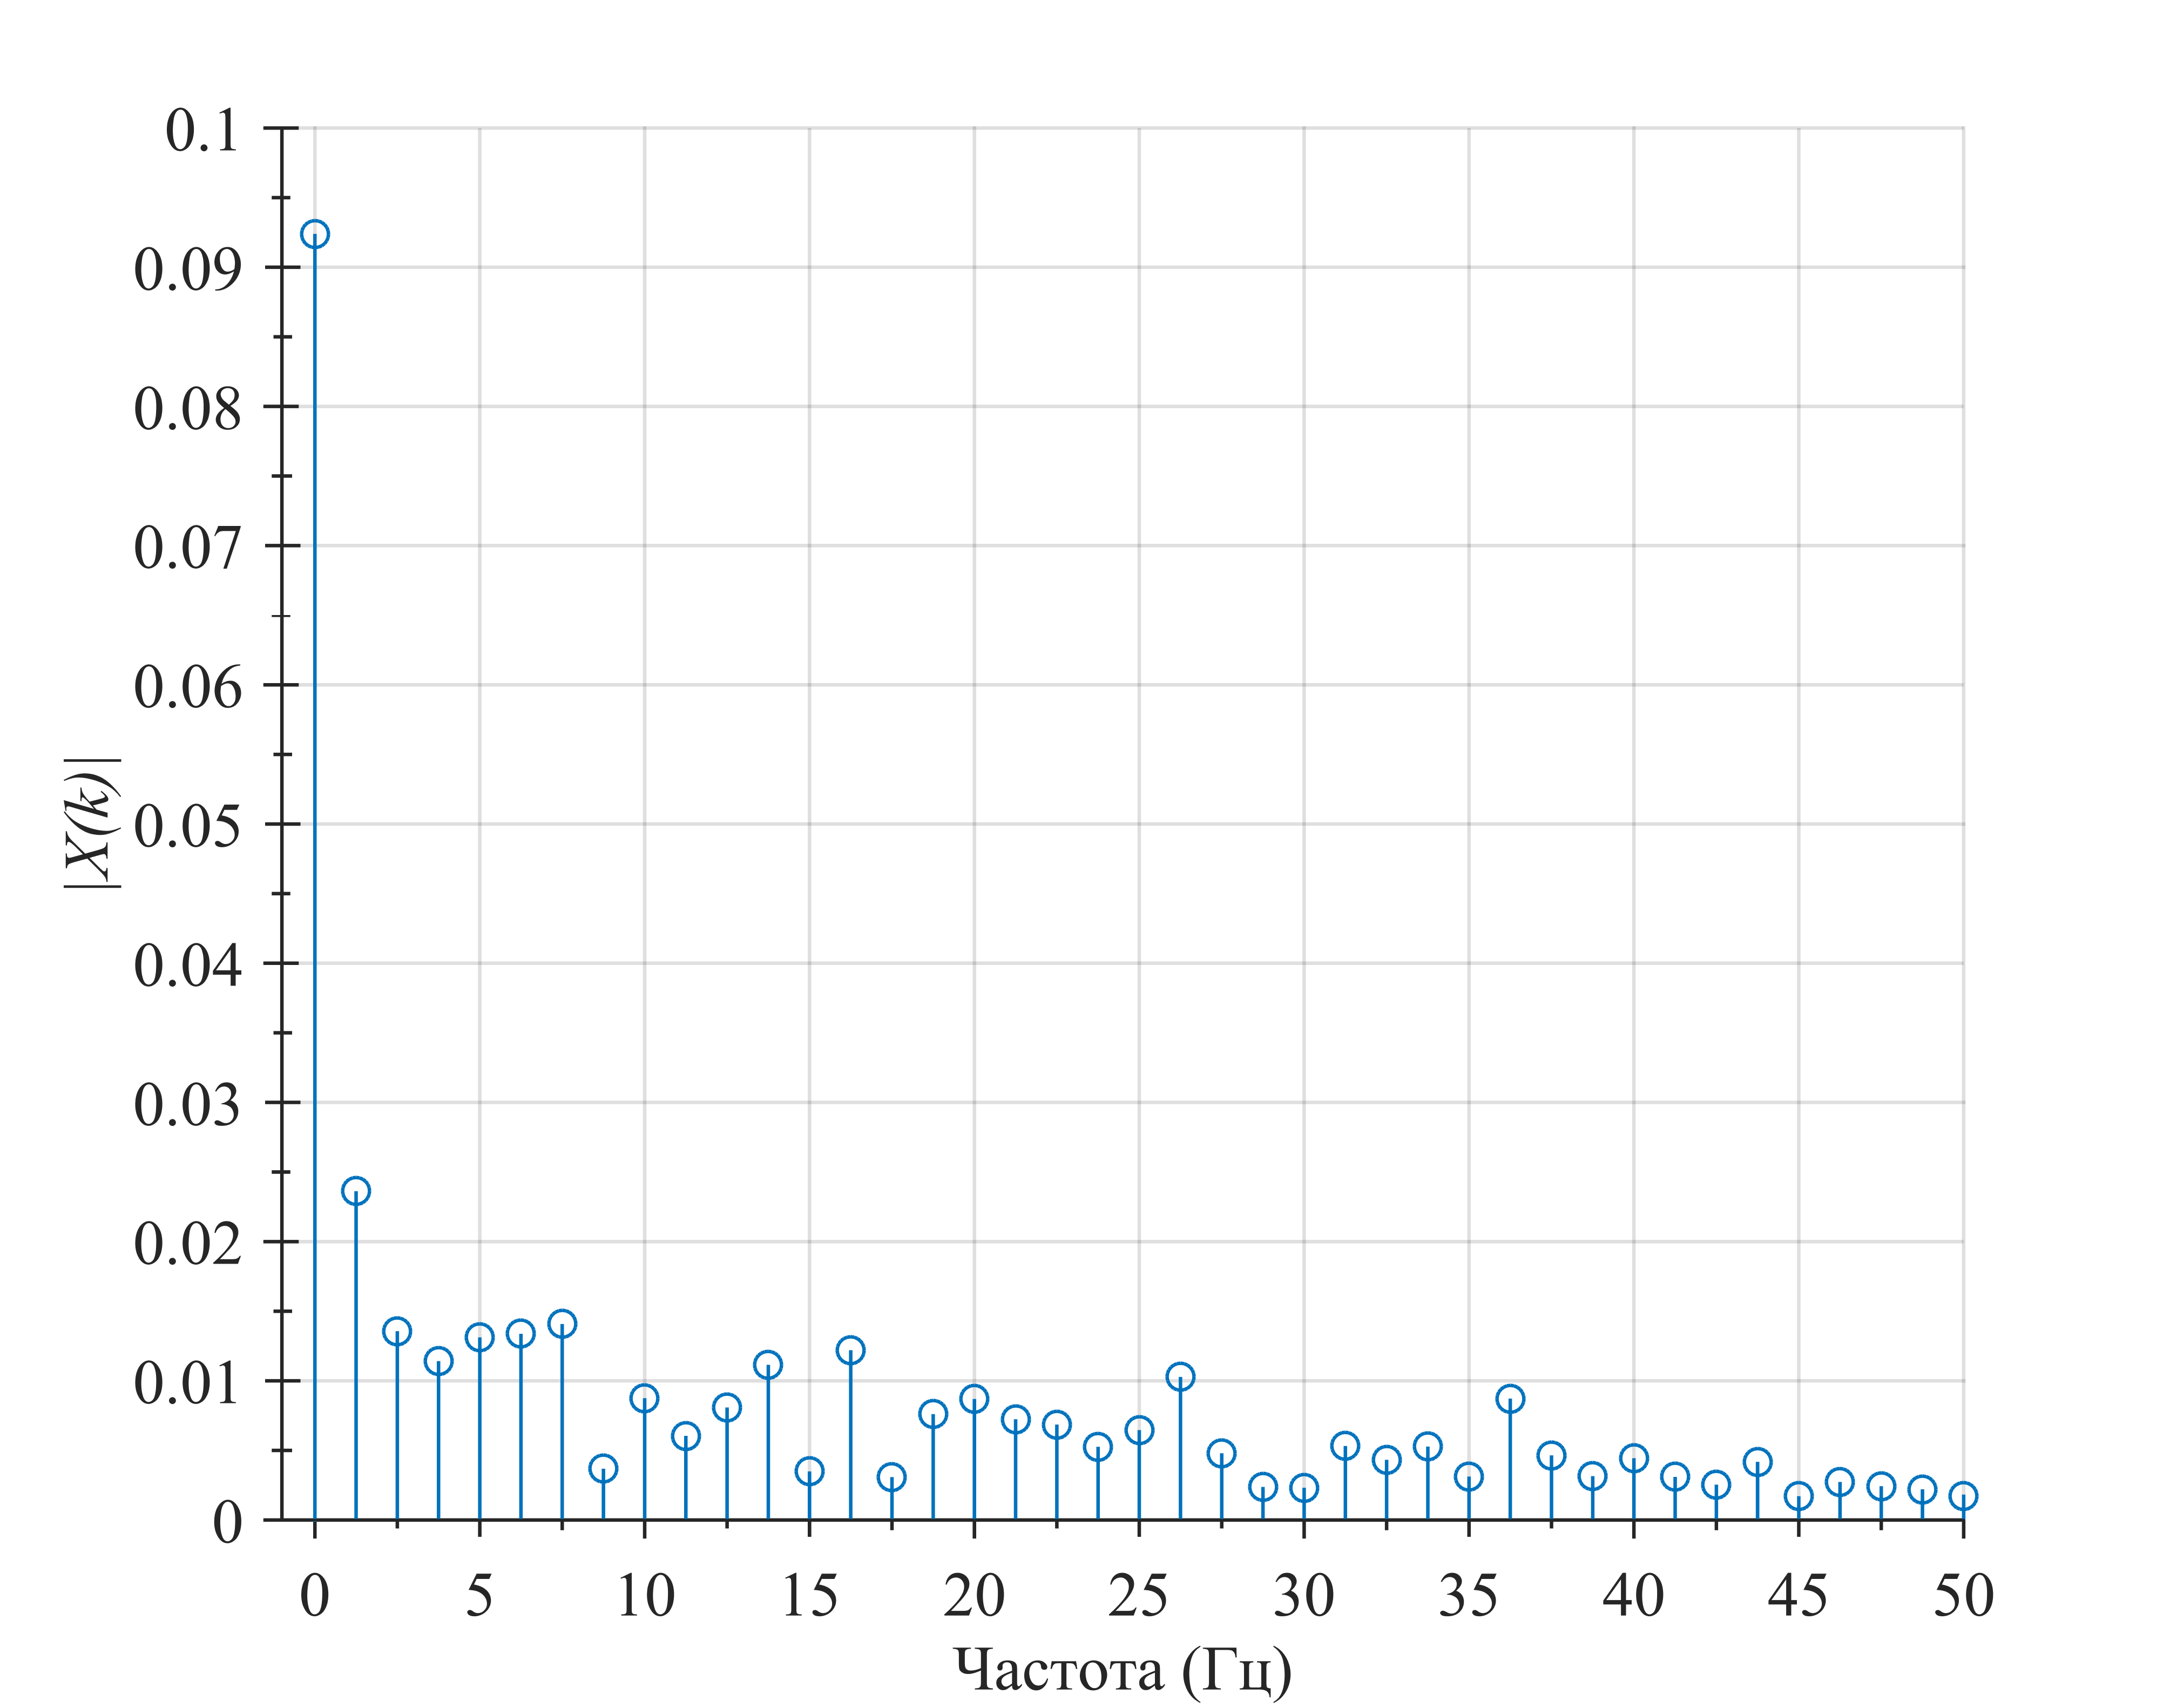
\includegraphics[width=\textwidth]{Spectrum}
	\caption{Спектр сигнала переходного процесса разрушения льда, для горизонтальной составляющей силы. При $ R=0,5 $ и $ t=10 $} 
	\label{img:Spectrum}  
\end{figure}

Как видно из рисунка \ref{img:Spectrum} при нулевой частоте заметен значительный всплеск амплитуды. Что обуславливает присутствие в сигнале некой постоянной составляющей с амплитудой равной 0,0926.  Для ее удаления из сигнала достаточно просто обнулить первый элемент в полученном ряду Фурье (значение амплитуда для составляющей с частотой 0, тоесть постоянной) \lstinline{X(1)=0;} и выполнить обратное преобразование с помощью формулы:
\begin{equation}\label{eq:iFFT}
x(j)=\frac{1}{N}\sum_{k=1}^{N} X(k)\cdot\omega_{N}
\end{equation}

Средствами matlab это же действие выполняется путем обратного сдвига и обратного же БПФ:
\begin{lstlisting}[stepnumber=0]
X = ifftshift(X);
x = ifft(X);
\end{lstlisting}
\begin{figure}[ht] 
	\center
	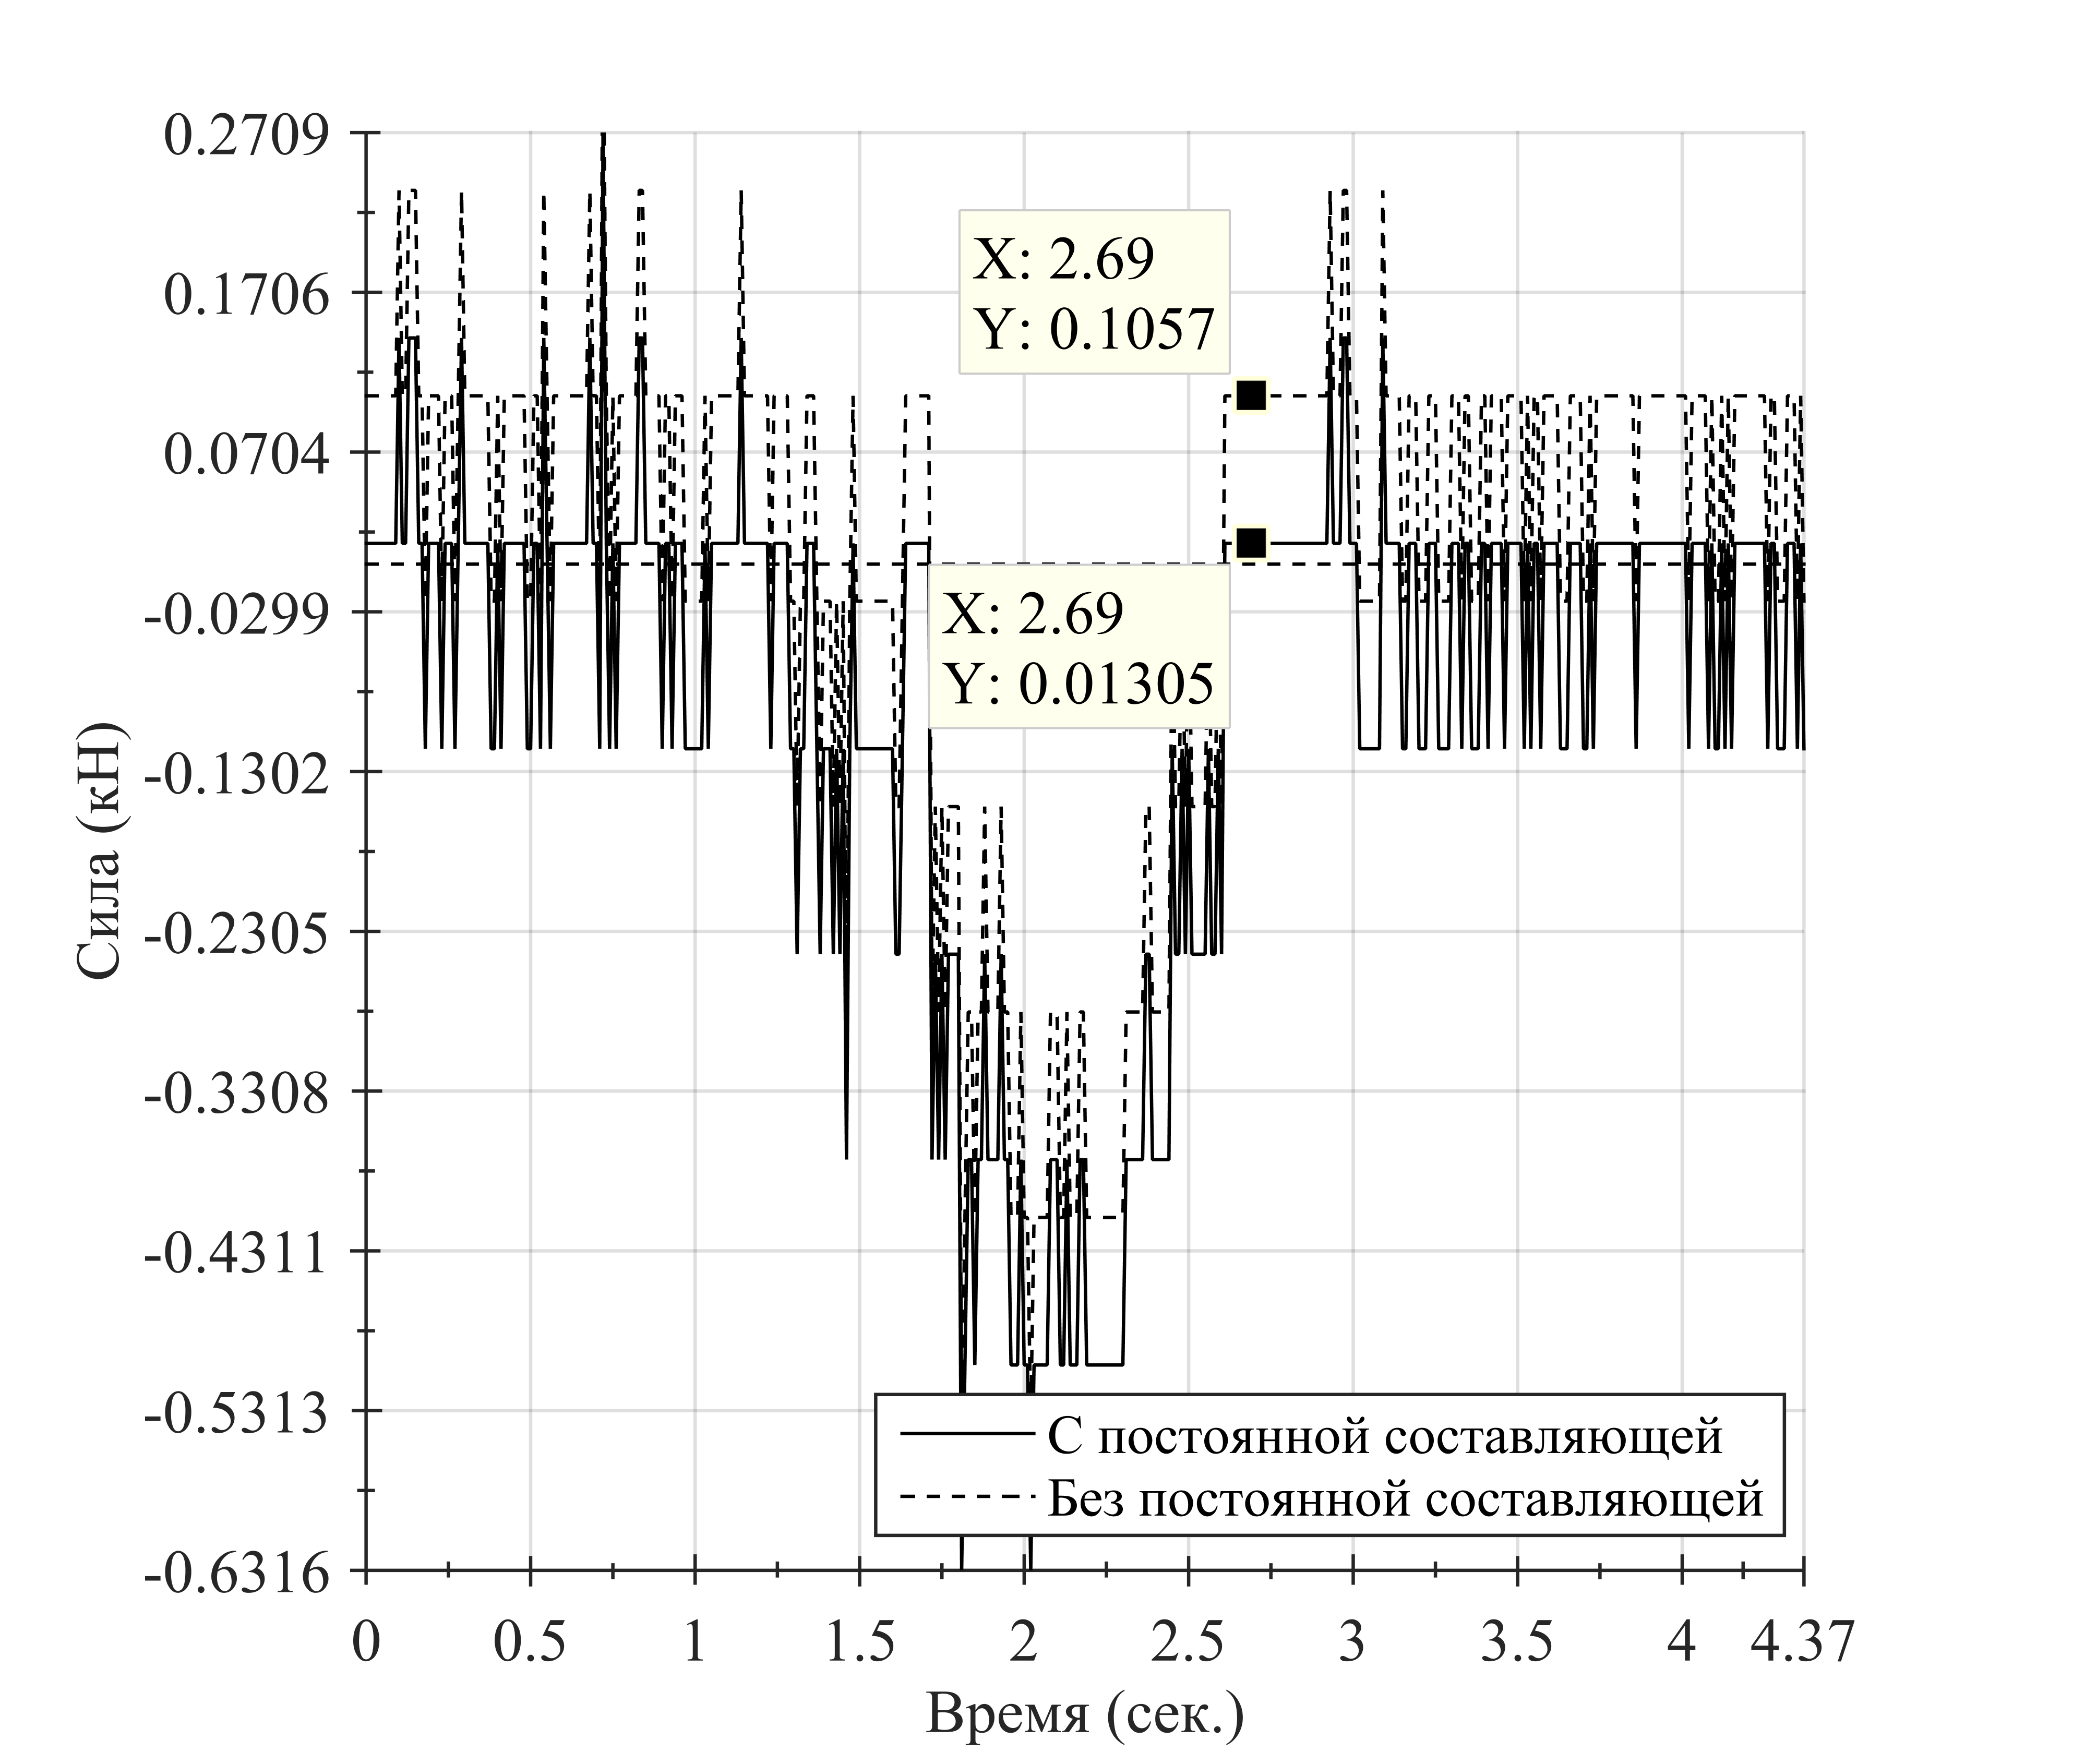
\includegraphics[width=\textwidth]{SignalRaw}
	\caption{Переходный процесса разрушения льда} 
	\label{img:SignalRaw}  
\end{figure}

Результат работы данного алгоритма приведен на рисунке \ref{img:SignalRaw}. Как видно из графика, не обработанный сигнал (сплошная линия) имеет смещение относительно обработанного (штриховая линия) ровно на 0,0926 что соответствует амплитуде постоянной составляющей, найденной выше. Все остальные записанные сигналы обработаем подобным образом.

Алгоритм реализованный средствами пакета прикладных программ matlab представлен в приложении \ref{Appendix:FPE:COF}, листинг \ref{list:clearOffSet}.



\section{Усреднение данных повторных опытов}\label{sect:mean_data}

В данном параграфе рассматривается три вида усреднения:
\begin{itemize}
	\item фильтрация сигнала с помощью метода скользящего среднего;
	\item усреднение сигнала переходного процесса, получение его действующего значения;
	\item усреднение действующих значений сигналов переходных процессов повторных опытов.
\end{itemize}

В задачах контроля технологических процессов важно знать энергетические свойства переменного сигнала, характеризующие его способность совершать работу. Таким параметром является его действующее значение. Мы будем вычислять именно его а не максимальное значение, так как нельзя с уверенность сказать что на всем промежутке времени переходного процесса сила действующая на резец будет постоянна. Однако, действующее значение будет учитывать нарастание и спад усилия при внедрении и выходе режущего инструмента из массива соответственно. При скорости резания $ 0,5\ \slantfrac{\textbf{м}}{\text{с}} $ такое влияние будет минимальным, поэтому им можно пренебречь.
\begin{equation}\label{eq:rms}
F_\text{Д}=\sqrt{\frac{1}{n}\cdot\sum_{i=1}^{n} F_i}
\end{equation}
где $ n $ "--- количество измерений в сигнале переходного процесса, $ F_i $ "--- измеренное значение в отдельном опыте.

Если мы будем рассматривать сигнал, например вертикальной составляющей \todo{вставить ссылку на рисунок сглаженного сигнала}, можно заметить интервалы времени при которых значение силы либо равно 0, либо близко к нему. Это участки движения резца до внедрения в ледяной массив и после выхода из него. Если мы будем расчитывать действующее значение силы по всему сигналу переходного процесса резания льда, то такие участки значительно занизят значение истинной величины силы. Предлагается отбросить их путем введения зоны не чувствительности 15\% от максимального значения сигнала относительно нуля.

\todo{График показывающий действующее значение и зону нечувствительности}

Такую операцию произведем с каждым из переходных процессов полученных в ходе экспериментальных исследований. Результаты вычислений сведем в таблицу:
\begin{table} [htbp]%
	\centering
	\captionsetup{width=\textwidth}
	\caption{Действующие значения вертикальной составляющих силы сопротивления резанию}%
	\label{tbl:RezD}% label всегда желательно идти после caption
	\begin{tabularx}{\textwidth}{| m{5cm} *{5}{|X} |}
		\hline
		Показатель & \multicolumn{5}{c |}{Действующее значение силы ($ F_\text{Д} $), кН}\tabularnewline
		\hline
		Шаг резания ($ t $), мм &  \textbf{10} &  \textbf{20} & \textbf{30} & \textbf{40} & \textbf{50} \tabularnewline
		\hline
		\hline
		Опыт №1 &  0 &  0 &  0 &  0 &  0 \tabularnewline
		Опыт №2 &  0 &  0 &  0 &  0 &  0 \tabularnewline
		Опыт №3 &  0 &  0 &  0 &  0 &  0 \tabularnewline
		Опыт №4 &  0 &  0 &  0 &  0 &  0 \tabularnewline
		Опыт №5 &  0 &  0 &  0 &  0 &  0 \tabularnewline
		\hline
	\end{tabularx}%
\end{table}

Из параграфа \ref{sect2_2} известно, что для каждый опыт повторялся 5 раз, для учета неизвестных факторов, а это значит что данные необходимо усреднить. Точечную оценку величины действующей силы можно вычислить через \cite{Zajigaev}:
\begin{equation}\label{eq:x_ocenka}
\hat{F_\text{Д}}=\frac{1}{m}\sum_{i=1}^{m} {F_\text{Д}}_i,
\end{equation}
где $ n $ "--- число повторных опытов.

Среднеквадратичное отклонение точечной оценки Оценить точность позволит относительная погрешность измерений, вычисляемая по следующее формуле:
\begin{equation}\label{eq:Error}
\varepsilon=\frac{1}{n}\sum_{i=1}^{n} \frac{\left| x_i-\bar{x}\right| }{\bar{x}}\cdot100\%
\end{equation}